\documentclass[11pt,a4paper]{article}
\usepackage[T1]{fontenc}
\usepackage{lmodern}
\usepackage[spanish]{babel}
\usepackage[margin=2.5cm]{geometry}
\usepackage{booktabs,tabularx,graphicx,hyperref,enumitem,parskip}
\hypersetup{hidelinks}
\setlength{\parskip}{0.6em}
\begin{document}

{\LARGE\bfseries Proyecto final: clasificación visual de productos para Lokora\par}\vspace{0.4em}
\noindent \textbf{Avance III (R2-A3-S13). Implementación y pruebas}\par
\noindent Universidad de Cundinamarca. Posgrado. Aplicaciones en Deep Learning (608145)\par
\noindent Docente: Wilson Mauro Rojas Reales\par
\noindent Estudiante: Harold Duque (trabajo individual)\par
\noindent Fecha: 17 de noviembre de 2026\par
\section*{Resumen}
\noindent Se entrenó y evaluó MobileNetV2 con aprendizaje por transferencia para sugerir una de tres categorías de producto (envasados, frutas, verduras) a partir de una fotografía. El modelo se comparó con dos referencias: predecir la clase más frecuente y una regresión logística sobre histogramas de color. MobileNetV2 obtuvo un macro-F1 de 0,969 en validación y de 0,969 en prueba, frente a 0,514 y 0,664 de la regresión logística. Los errores se concentran entre frutas y verduras. Estos resultados provienen de un conjunto público cuyos metadatos no permiten garantizar independencia entre particiones ni representan aún fotografías de vendedores de Lokora; por eso se tratan como evidencia preliminar y no como desempeño esperado en producción.\par
\section*{1. Implementación}
\noindent \textbf{Datos.} Grocery Store Dataset (Klasson et al., 2019), usando solo fotografías naturales y sus listas oficiales de partición: 2.640 imágenes de entrenamiento, 296 de validación y 2.485 de prueba. Las carpetas Fruit, Vegetables y Packages se mapean a frutas, verduras y envasados.\par
\noindent \textbf{Modelo.} MobileNetV2 preentrenada en ImageNet, con la base congelada y una cabeza nueva: pooling global, dropout de 0,2 y capa softmax de tres salidas. Las imágenes se orientan según EXIF, se convierten a RGB, se ajustan con relleno a 224 $\times$ 224 y se escalan de 0--255 a -1--1 dentro del modelo. El aumento de datos se aplica solo en entrenamiento.\par
\noindent \textbf{Entrenamiento.} Adam con tasa de 0,001, lotes de 32 y un máximo de 20 épocas con parada temprana (paciencia de cuatro épocas sobre la pérdida de validación). La parada temprana no se activó: la pérdida de validación siguió mejorando y se completaron las 20 épocas. El entrenamiento tomó 387 segundos en una GPU Tesla T4 de Google Colab.\par
\begin{center}\small
\begin{tabularx}{\textwidth}{XX}
\toprule
\textbf{Elemento} & \textbf{Valor} \\
\midrule
Semilla & 42 \\
Python / TensorFlow & 3.13.16 / 2.21.0 \\
scikit-learn / NumPy / pandas & 1.6.1 / 2.4.6 / 2.2.3 \\
Identificador del run & 20261118T011749179143Z \\
Artefactos & modelo.keras, métricas, predicciones, historial, manifiesto con particiones y hashes \\
\bottomrule
\end{tabularx}
\end{center}
\noindent \textbf{Trazabilidad.} Cada ejecución guarda el manifiesto con SHA-256, versiones de las bibliotecas, parámetros, historial, predicciones y el hash del artefacto. Los archivos están en la carpeta \texttt{resultados/mobilenetv2/} del repositorio (\url{https://github.com/HaroldDuke/lokora-clasificacion-productos}).\par
\section*{2. Pruebas}
\noindent \textbf{Protocolo.} Los modelos se compararon en validación. La partición de prueba se calculó al final del run, sin ajustar hiperparámetros con ella. La métrica principal es macro-F1, que da el mismo peso a las tres clases; se reportan también exactitud, precisión y recall por clase.\par
\begin{center}\small
\begin{tabularx}{\textwidth}{>{\raggedright\arraybackslash}p{0.28\textwidth}>{\raggedleft\arraybackslash}p{0.145\textwidth}>{\raggedleft\arraybackslash}p{0.145\textwidth}>{\raggedleft\arraybackslash}p{0.145\textwidth}>{\raggedleft\arraybackslash}p{0.145\textwidth}}
\toprule
\textbf{Modelo} & \textbf{Exactitud (val.)} & \textbf{Macro-F1 (val.)} & \textbf{Exactitud (prueba)} & \textbf{Macro-F1 (prueba)} \\
\midrule
Clase más frecuente & 0,3750 & 0,1818 & 0,4495 & 0,2067 \\
Histograma RGB y regresión logística & 0,5304 & 0,5136 & 0,6809 & 0,6642 \\
\textbf{MobileNetV2 con transferencia} & \textbf{0,9696} & \textbf{0,9689} & \textbf{0,9718} & \textbf{0,9694} \\
\bottomrule
\end{tabularx}
\end{center}
\noindent MobileNetV2 supera con claridad a las dos referencias en ambas particiones, por lo que su uso queda justificado frente a ellas. La meta exploratoria de macro-F1 en prueba de 0,80 se cumple, pero era un criterio provisional.\par
\noindent \textbf{Resultados por clase de MobileNetV2 en prueba.}\par
\begin{center}\small
\begin{tabularx}{\textwidth}{>{\raggedright\arraybackslash}p{0.28\textwidth}>{\raggedleft\arraybackslash}p{0.145\textwidth}>{\raggedleft\arraybackslash}p{0.145\textwidth}>{\raggedleft\arraybackslash}p{0.145\textwidth}>{\raggedleft\arraybackslash}p{0.145\textwidth}}
\toprule
\textbf{Clase} & \textbf{Precisión} & \textbf{Recall} & \textbf{F1} & \textbf{Imágenes} \\
\midrule
Envasados & 1,000 & 1,000 & 1,000 & 781 \\
Frutas & 0,958 & 0,980 & 0,969 & 1.117 \\
Verduras & 0,961 & 0,918 & 0,939 & 587 \\
\bottomrule
\end{tabularx}
\end{center}
\noindent \textbf{Matriz de confusión en prueba} (filas: clase real; columnas: clase predicha).\par
\begin{center}\small
\begin{tabularx}{\textwidth}{>{\raggedright\arraybackslash}p{0.28\textwidth}>{\raggedleft\arraybackslash}p{0.193\textwidth}>{\raggedleft\arraybackslash}p{0.193\textwidth}>{\raggedleft\arraybackslash}p{0.193\textwidth}}
\toprule
\textbf{Real \textbackslash{} Predicha} & \textbf{Envasados} & \textbf{Frutas} & \textbf{Verduras} \\
\midrule
Envasados & 781 & 0 & 0 \\
Frutas & 0 & 1.095 & 22 \\
Verduras & 0 & 48 & 539 \\
\bottomrule
\end{tabularx}
\end{center}
\begin{figure}[htbp]\centering
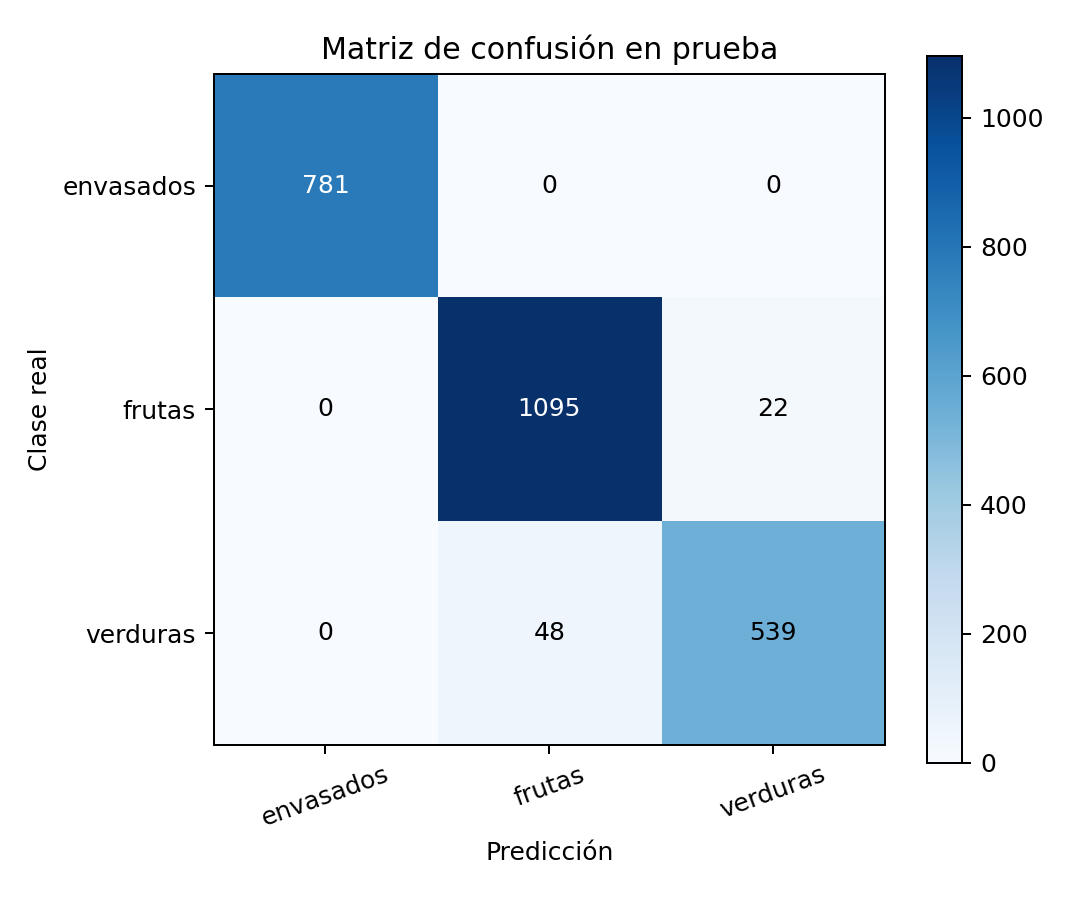
\includegraphics[width=0.92\textwidth]{figuras/matriz_confusion.png}
{\small Figura 1. Matriz de confusión de MobileNetV2\par}
\end{figure}
\begin{figure}[htbp]\centering
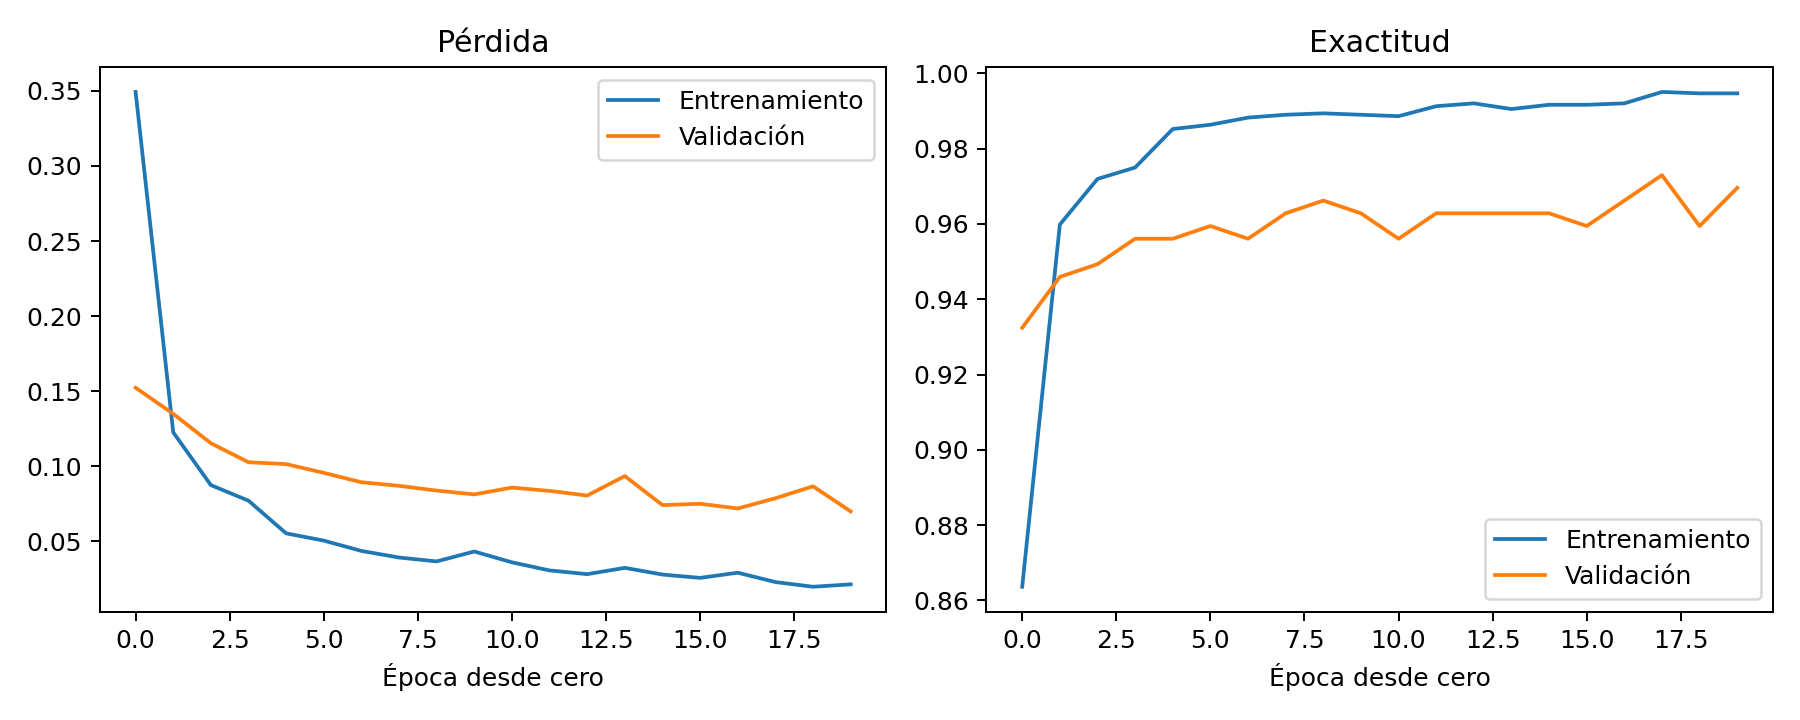
\includegraphics[width=0.92\textwidth]{figuras/curvas_entrenamiento.png}
{\small Figura 2. Curvas de pérdida y exactitud durante el entrenamiento\par}
\end{figure}
\noindent Las curvas muestran que la pérdida de validación baja de 0,152 a 0,070. Al final, la exactitud de entrenamiento es de 0,995 y la de validación de 0,970. Esa brecha indica un sobreajuste leve que no impide un buen desempeño en prueba (0,972).\par
\section*{3. Análisis de errores}
\noindent De las 2.485 imágenes de prueba, 70 se clasificaron mal (2,8 \%): 48 verduras predichas como frutas y 22 frutas predichas como verduras. Ningún envasado se confundió. Los productos con más errores, tomados de la ruta de cada imagen en el conjunto, son:\par
\begin{center}\small
\begin{tabularx}{\textwidth}{XrrX}
\toprule
\textbf{Producto} & \textbf{Errores} & \textbf{Imágenes de prueba} & \textbf{Confusión} \\
\midrule
Pimiento (Pepper) & 13 & 110 & verdura $\rightarrow$ fruta \\
Repollo (Cabbage) & 8 & 19 & verdura $\rightarrow$ fruta \\
Cebolla (Onion) & 8 & 37 & verdura $\rightarrow$ fruta \\
Kiwi & 7 & 45 & fruta $\rightarrow$ verdura \\
Papa (Potato) & 7 & 70 & verdura $\rightarrow$ fruta \\
Banano (Banana) & 6 & 44 & fruta $\rightarrow$ verdura \\
Maracuyá (Passion-Fruit) & 4 & 27 & fruta $\rightarrow$ verdura \\
\bottomrule
\end{tabularx}
\end{center}
\noindent La confianza media (softmax máximo) es de 0,987 en los aciertos y de 0,804 en los errores. Sin embargo, 27 de los 70 errores tienen una confianza de 0,9 o más, así que la puntuación por sí sola no basta para decidir cuándo pedir una revisión adicional al vendedor. Las salidas softmax no tienen calibración demostrada.\par
\section*{4. Limitaciones}
\begin{enumerate}[nosep]
\item \textbf{Independencia entre particiones.} Los metadatos del conjunto no identifican el objeto físico ni la sesión de captura. Fotografías casi idénticas del mismo producto pueden estar repartidas entre entrenamiento y prueba, lo que puede inflar las métricas. No se afirma independencia por producto.
\item \textbf{Cambio de dominio.} Las fotografías son de tienda, tomadas con teléfono. No se han probado fotografías reales de vendedores de Lokora.
\item \textbf{Alcance.} Solo tres categorías y un producto principal por imagen. El modelo no detecta de forma fiable productos ajenos a ellas.
\item \textbf{Convenciones de etiquetado.} Algunos productos son ambiguos (el tomate, por ejemplo, sigue la convención del conjunto y se etiqueta como verdura).
\item \textbf{Latencia.} La latencia de inferencia reportada por el run es de 159 ms de mediana y 173 ms en el percentil 95, medida solo sobre un tensor ya preparado. No incluye carga de la imagen, red ni servicio. Debe medirse de nuevo en el despliegue.
\end{enumerate}
\section*{5. Rediseño propuesto}
\noindent Las pruebas sugieren estas modificaciones, que se evaluarán en los siguientes avances y no se han implementado todavía:\par
\begin{center}\small
\begin{tabularx}{\textwidth}{XXX}
\toprule
\textbf{Cambio} & \textbf{Motivo} & \textbf{Evidencia que lo motiva} \\
\midrule
Agrupar por producto o sesión en fotografías propias & Evitar fugas entre particiones & Limitación 1 \\
Evaluar con fotografías de vendedores de Lokora & Medir el cambio de dominio & Limitación 2 \\
Ajuste fino de las últimas capas de MobileNetV2 & Reducir errores entre frutas y verduras & Sección 3 \\
Probar un modelo basado en Transformers (por ejemplo ViT o CLIP) como segunda alternativa & Comparar con un enfoque distinto & Revisión de literatura (Avance I) \\
Incorporar el nombre del producto como entrada de texto & Resolver casos ambiguos como el pimiento o el tomate & Sección 3 y Zahavy et al. (2016) \\
Umbral de confianza y confirmación del vendedor & Gestionar errores con alta confianza & Sección 3 \\
\bottomrule
\end{tabularx}
\end{center}
\section*{6. Siguientes pasos}
\begin{center}\small
\begin{tabularx}{\textwidth}{XX}
\toprule
\textbf{Entrega} & \textbf{Contenido} \\
\midrule
Avance IV (23 de noviembre) & Modelo escogido, modelos probados, herramientas y métricas con la interpretación de resultados \\
Avance V y proyecto final (25 de noviembre) & Comparación con el desempeño de una persona, despliegue en la nube con interfaz o API y socialización \\
\bottomrule
\end{tabularx}
\end{center}
\section*{Referencias}
\noindent [1] Klasson, M., Zhang, C. y Kjellström, H. (2019). A Hierarchical Grocery Store Image Dataset with Visual and Semantic Labels. IEEE Winter Conference on Applications of Computer Vision (WACV). \url{https://arxiv.org/abs/1901.00711}\par
\noindent [2] Sandler, M., Howard, A., Zhu, M., Zhmoginov, A. y Chen, L.-C. (2018). MobileNetV2: Inverted Residuals and Linear Bottlenecks. CVPR. \url{https://arxiv.org/abs/1801.04381}\par
\noindent [3] Zahavy, T., Magnani, A., Krishnan, A. y Mannor, S. (2016). Is a picture worth a thousand words? A Deep Multi-Modal Fusion Architecture for Product Classification in e-commerce. \url{https://arxiv.org/abs/1611.09534}\par
\noindent [4] Keras. Transfer learning and fine tuning. \url{https://keras.io/guides/transfer_learning/}\par
\end{document}
